\documentclass[tikz,border=2pt]{standalone}
\usepackage{amsmath}
\usepackage{tikz}
\usetikzlibrary{arrows.meta}

\begin{document}
% Injective: distinct inputs never share an output (left). Not injective: two arrows meet (right).
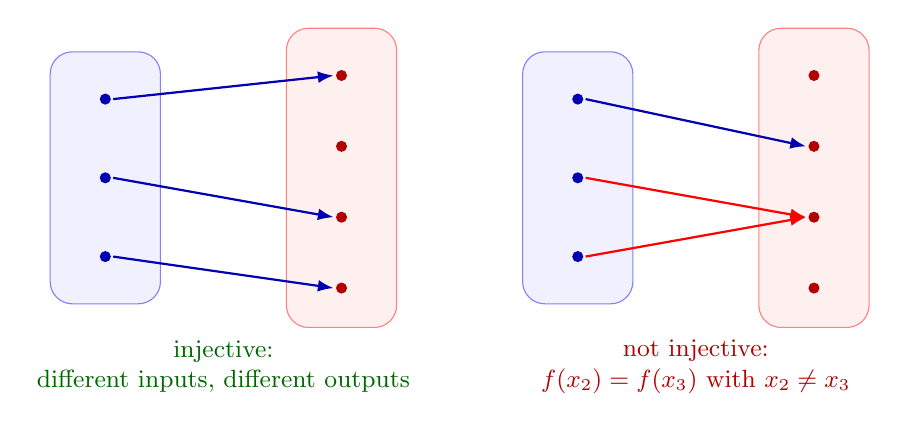
\begin{tikzpicture}[>={Latex[length=2mm]}, every node/.style={font=\small}]
	\begin{scope}
		\draw[rounded corners=8pt, fill=blue!6, draw=blue!50] (-0.7,-1.6) rectangle (0.7,1.6);
		\draw[rounded corners=8pt, fill=red!6, draw=red!50] (2.3,-1.9) rectangle (3.7,1.9);
		\foreach \y in {1.0,0,-1.0} {\fill[blue!70!black] (0,\y) circle (2pt);}
		\foreach \y in {1.3,0.4,-0.5,-1.4} {\fill[red!70!black] (3,\y) circle (2pt);}
		\draw[->, blue!70!black, thick] (0.1,1.0) -- (2.9,1.3);
		\draw[->, blue!70!black, thick] (0.1,0) -- (2.9,-0.5);
		\draw[->, blue!70!black, thick] (0.1,-1.0) -- (2.9,-1.4);
		\node[green!40!black, align=center] at (1.5,-2.4) {injective:\\ different inputs, different outputs};
	\end{scope}
	\begin{scope}[xshift=6cm]
		\draw[rounded corners=8pt, fill=blue!6, draw=blue!50] (-0.7,-1.6) rectangle (0.7,1.6);
		\draw[rounded corners=8pt, fill=red!6, draw=red!50] (2.3,-1.9) rectangle (3.7,1.9);
		\foreach \y in {1.0,0,-1.0} {\fill[blue!70!black] (0,\y) circle (2pt);}
		\foreach \y in {1.3,0.4,-0.5,-1.4} {\fill[red!70!black] (3,\y) circle (2pt);}
		\draw[->, blue!70!black, thick] (0.1,1.0) -- (2.9,0.4);
		\draw[->, red, thick] (0.1,0) -- (2.9,-0.5);
		\draw[->, red, thick] (0.1,-1.0) -- (2.9,-0.5);
		\node[red!70!black, align=center] at (1.5,-2.4) {not injective:\\ $f(x_2)=f(x_3)$ with $x_2\neq x_3$};
	\end{scope}
\end{tikzpicture}
\end{document}
